\documentclass[a4paper, twocolumn]{article}
\usepackage{lipsum}
\usepackage{graphicx}
\usepackage{subcaption}
\usepackage{tikz}
\usetikzlibrary[circuits.logic.CDH]

\title{Figures, Diagrams and Tables}
\author{Gary}

\begin{document}
\maketitle	

\begin{abstract}
	\lipsum[1]
\end{abstract}

\tableofcontents

\section{Introduction}
\lipsum[1-5]

\section{Figures}\label{sect:figures}
In Figure \ref{fig:cat} we see a cat. 

\lipsum[1-3]

\begin{figure}[tbp]
	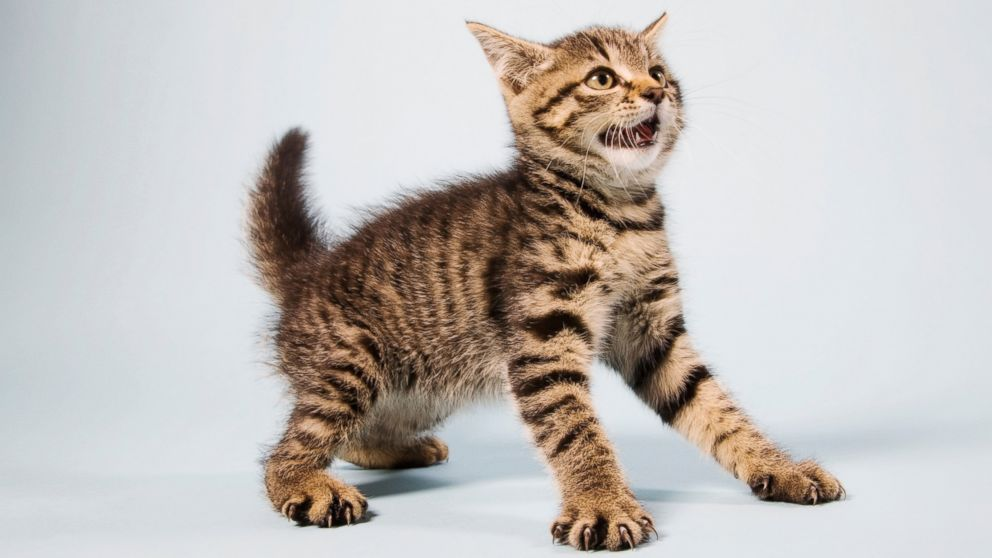
\includegraphics[width=\linewidth]{Figures/cat}
	\caption{This is a cat}
	\label{fig:cat}
\end{figure}


\begin{figure*}[tbp]
	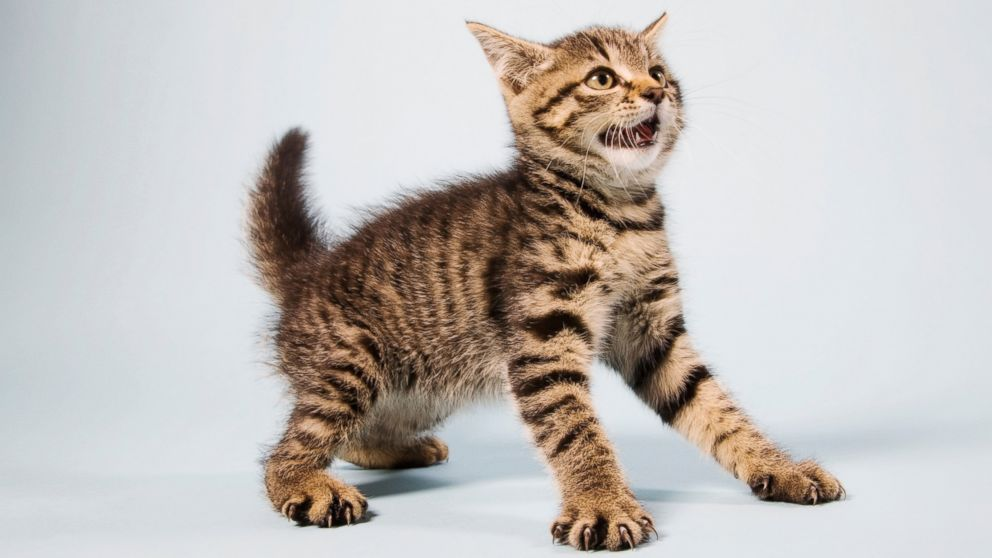
\includegraphics[width=\linewidth]{Figures/cat}
	\caption{This is a cat}
	\label{fig:big_cat}
\end{figure*}

\lipsum[1-17]

\begin{figure}
	\begin{subfigure}{0.16\textwidth}
		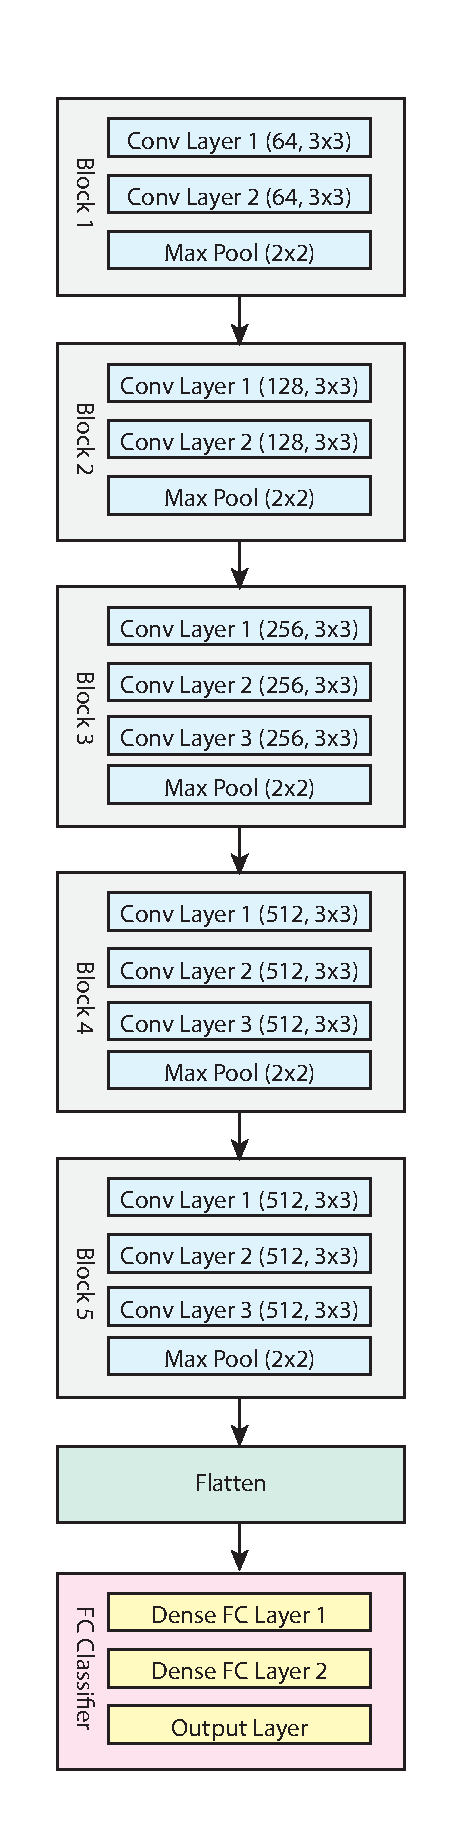
\includegraphics[width=\linewidth]{Figures/vgg_architecture}
		\caption{VGG Architecture}
		\label{fig:vgg}
	\end{subfigure}%
	\begin{subfigure}{0.16\textwidth}
		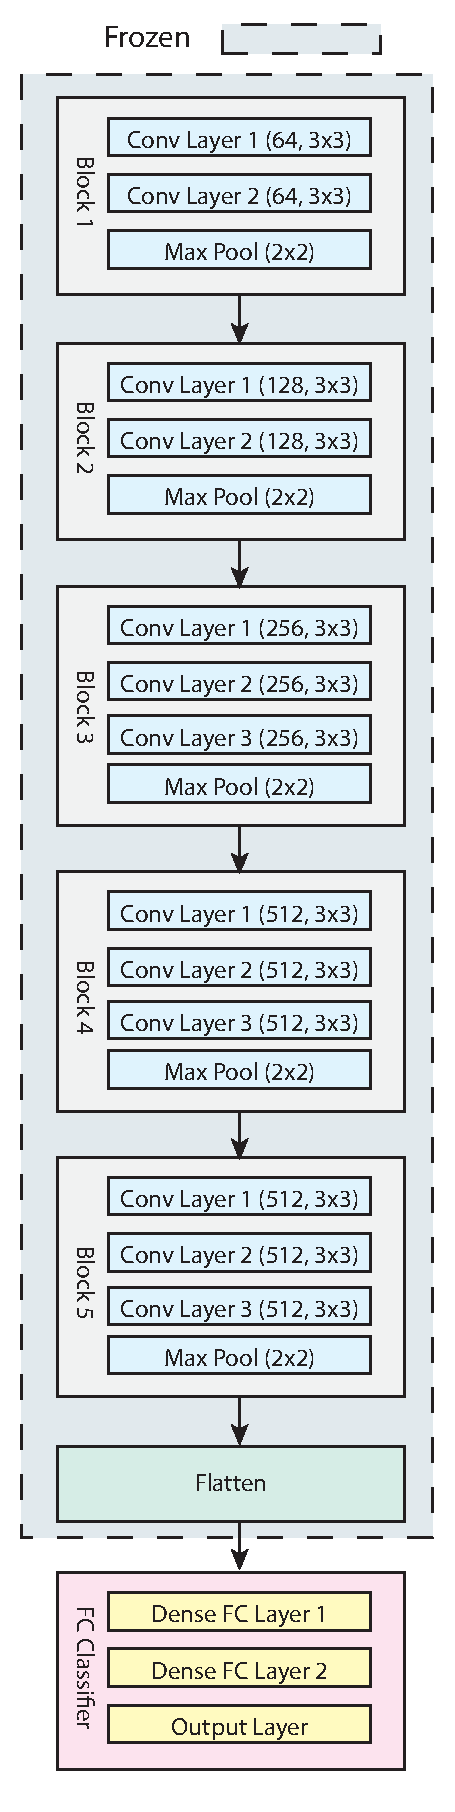
\includegraphics[width=\linewidth]{Figures/vgg_architecture_feature}
		\caption{VGG Feature Extraction }
		\label{fig:vgg2}
	\end{subfigure}%
	\begin{subfigure}{0.16\textwidth}
		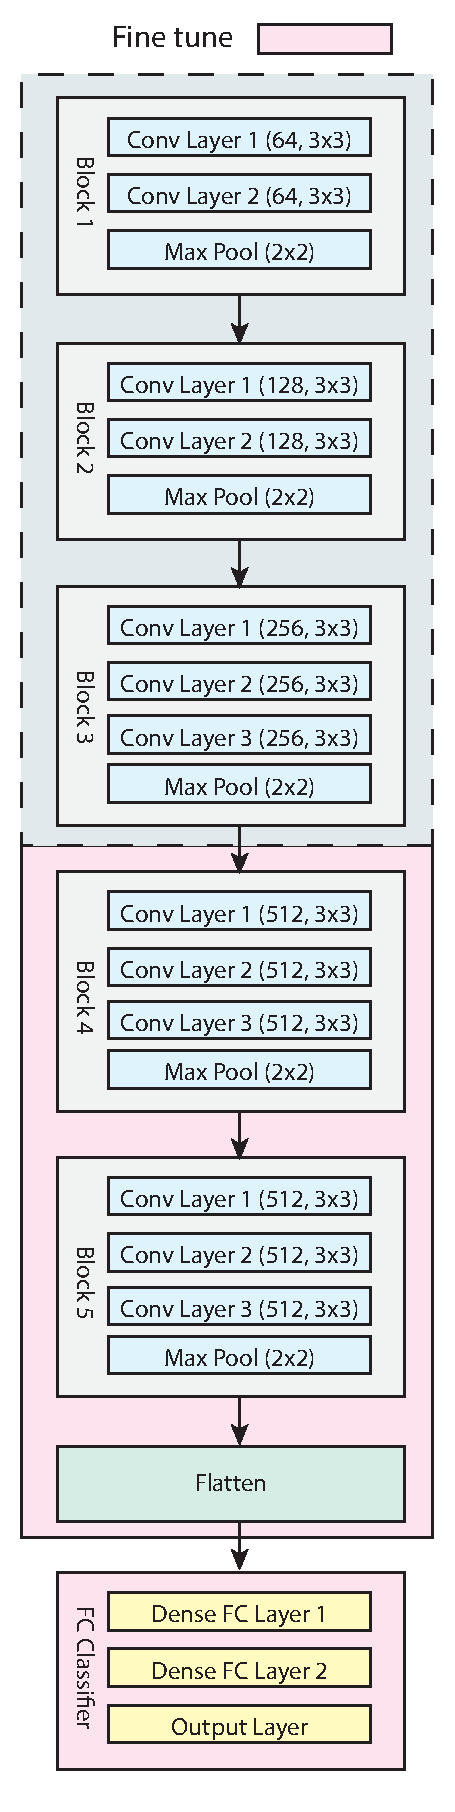
\includegraphics[width=\linewidth]{Figures/vgg_architecture_fine}
		\caption{VGG Fine Tuning}
		\label{fig:vgg3}
	\end{subfigure}%
	\caption{Collection of VGGs}
	\label{fig:vgg_overall}
\end{figure}

As seen in Figure \ref{fig:vgg}, \ref{fig:vgg2}  and in Figure \ref{fig:vgg_overall}.

\section{Plots}

\begin{tikzpicture}[scale=1]
\draw (0.0,0.0) rectangle (0.4,0.2);
\draw (0.0,0.0) -- (0.4,0.2);
\draw (0.0,0.2) -- (0.4,0.0);
\end{tikzpicture}

\lipsum[1-4]

\begin{figure}
	\centering
	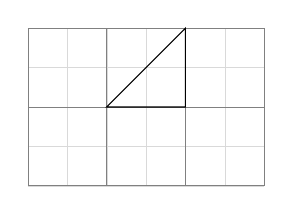
\begin{tikzpicture}
	\draw[line width=0.1pt,gray!30,step=5mm]
	(0,0) grid (3,2);
	\draw[help lines] (0,0) grid (3,2);
	\draw (1,1) -- (2,2) -- (2,1) -- cycle;
	\end{tikzpicture}
	\caption{Tikz Plot}
\end{figure}

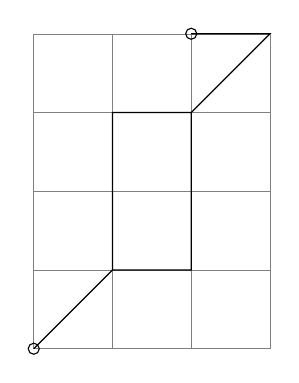
\begin{tikzpicture}
\draw[help lines] (0,0) grid (3,4);
\draw (0,0) circle (2pt)
-- (1,1) rectangle (2,3)
-- (3,4)
-- (2,4) circle (2pt);
\end{tikzpicture}

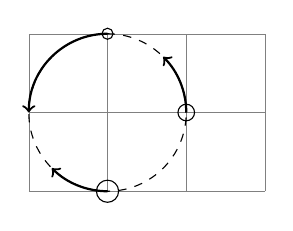
\begin{tikzpicture}
\draw[help lines] (0,0) grid (3,2);
\draw[dashed] (1,1) circle (1cm);
\draw (1,2) coordinate(a) circle (2pt)
(2,1) coordinate(b) circle (3pt)
(1,0) coordinate(c) circle (4pt);
\draw[->,thick] (a) arc (90:180:1cm);
\draw[->,thick] (b) arc (0:45:1cm);
\draw[->,thick] (c) arc (270:225:1cm);
\end{tikzpicture}

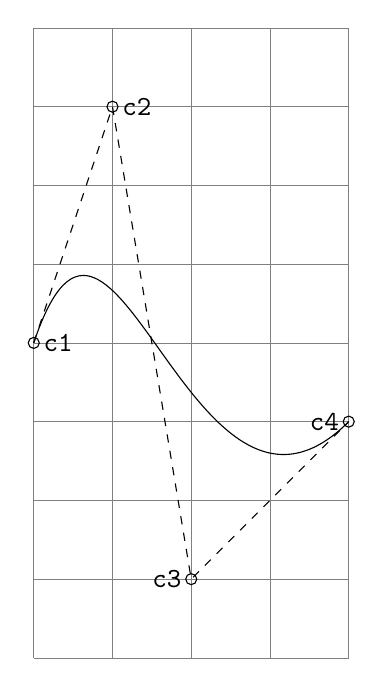
\begin{tikzpicture}
\draw[help lines] (-2,-4) grid (+2,+4);
\path (-2,+0) coordinate(c1)
(-1,+3) coordinate(c2)
(+0,-3) coordinate(c3)
(+2,-1) coordinate(c4);
\draw[dashed] (c1) -- (c2) -- (c3) -- (c4);
\draw (c1) circle (2pt)
(c2) circle (2pt)
(c3) circle (2pt)
(c4) circle (2pt)
(c1) .. controls (c2)
and (c3) .. (c4)
(c1) node[anchor=west] {\texttt{c1}}
(c2) node[anchor=west] {\texttt{c2}}
(c3) node[anchor=east] {\texttt{c3}}
(c4) node[anchor=east] {\texttt{c4}};
\end{tikzpicture}

\subsection{Colour}
\begin{tikzpicture}[color=red]
\draw (0,3) -- (2,3);
\draw[color=green, thick, ->] (0,2) -- (2,2);
\draw[color=cyan!50!red] (0,1) -- (2,1);
\end{tikzpicture}


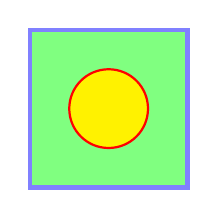
\begin{tikzpicture}[fill=blue!40,scale=1]
\filldraw[ultra thick,fill=green!50, draw=blue!50]
(0,0) rectangle (2,2);
\filldraw[thick,fill=yellow,draw=red]
(1,1) circle (0.5cm);
\end{tikzpicture}

\subsection{Trees}

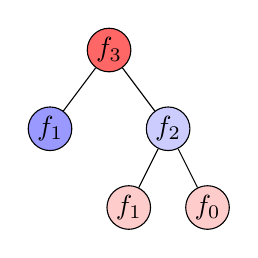
\begin{tikzpicture}
[level distance=10mm%
,every node/.style={fill=red!60,%
	circle,%
	draw=black,%
	inner sep=1pt}%
,level 1/.style={sibling distance=15mm},%
,level 2/.style={sibling distance=10mm,%
	nodes={fill=red!20}}]
\node (top) {$f_3$}
child {node[fill=blue!40] {$f_1$}}
child {node[fill=blue!20] {$f_2$}
	child {node {$f_1$}}
	child {node {$f_0$}}};
\end{tikzpicture}

\subsection{Circuit Diagram}
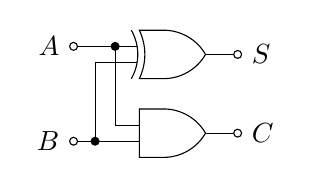
\begin{tikzpicture}
[circuit logic CDH,
circuit declare symbol=connection,
circuit declare symbol=io,
set connection graphic={fill=black,
	shape=circle,
	minimum size=1mm},
set io graphic={draw,shape=circle,
	minimum size=1mm},
every circuit symbol/.style={fill=white,draw}]
\draw node[xor gate] (x) {}
+(0,-1) node[and gate] (a) {}
(x.input 1) +(-0.8,0) node[io] (A) {}
(A |- a.input 2) node[io] (B) {}
(x.output) -- +(0.4,0) node[io] (S) {}
(a.output) -- (a.output -| S)
node[io] (C) {}
($(B)!0.33!(a.input 2)$) node[connection] {}
|- (x.input 2)
($(A)!0.66!(x.input 1)$) node[connection] {}
|- (a.input 1)
(A.west) node[anchor=east] {$A$}
(B.west) node[anchor=east] {$B$}
(S.east) node[anchor=west] {$S$}
(C.east) node[anchor=west] {$C$}
(A) -- (x.input 1)
(B) -- (a.input 2);
\end{tikzpicture}

\subsection{Tables}
\lipsum[1]

Table \ref{tab:reasoning_layers} shows the different .. 



\begin{table}[tbp]
	\centering
	\caption{Computing Layer Characteristics}
	\label{tab:reasoning_layers}
	\resizebox{0.5\textwidth}{!}{%
		\begin{tabular}{llll}
			\hline
			Charachteristics & IoT & Edge & Cloud \\ \hline
			Deployment & Distributed & Distributed & Centralised \\
			Components & Physical Devices & Edge nodes & Virtual  \\
			Computational & Very Limited & Limited & Unlimited \\
			Storage & Small & Limited & Unlimited \\
			Response Time & NA & Fast & Slow \\
			Big Data & Source & Process & Process \\
			QoS & NA & High & Medium \\
			Energy  & Low & Low & High \\
			\hline
		\end{tabular}
	}
\end{table}

\begin{table}
	\centering
	\begin{tabular}{||c|c|c||}
		\hline
		Col1 & Col2 & Col3 \\ \hline
		3.2 & 3.1 & 3.5 \\ \hline
		3.2 & 3.1 & 4.5 \\ \hline
		3.222 & 3.41 & 6.5 \\ \hline
		3.22 & 3.1 & 8.5 \\ \hline
	\end{tabular}
	\caption{Speed Race Results}
	\label{tab:speed_race}
\end{table}


\begin{table*}[tbp]
	\centering
	\caption{Urban Applications}
	\label{tab:reasoning_layers_3}
	\resizebox{\textwidth}{!}{%
		\begin{tabular}{llllll}
			\hline
			Urban Application & Data Type & Traffic Rate & Tolerable Delay & Number of IoT Devices & Criticalicty \\ \hline
			Waste Management & Historical Data & \textgreater{}= 100 MB per day & \textgreater 30 mins & \textgreater{}=1000-1million per city & Low \\
			Structural Health & Historical Data & \textgreater{}= 10 MB per day & \textgreater 30 mins & \textgreater{}=10-1000 per building & High \\
			Air Quality Monitoring & Historical Data & \textgreater{}= 10 MB per day & \textgreater 30 mins & \textgreater{}=1000-1million per city & High \\
			Noise Monitoring & Historical Data & \textgreater{}= 100 MB per day & \textgreater 30 mins & \textgreater{}=1000-1million per city & Medium \\
			Wearable IoT & Stream Data & \textless{}=1 GB per device & \textgreater 30 mins & \textgreater{}=1-10 per person & Medium \\
			Traffic Congestion & Historical Data & \textgreater{}= 100 MB per day & \textgreater 5 mins & \textgreater{}=1000-1million per city & Low \\
			Smart Parking & Event Data & \textgreater{}= 10 MB per day & \textgreater 1 min & \textgreater{}=1000-1million per city & Low \\
			Smart Home & Stream/ Massive Data & \textgreater{}= 10 MB per house per day & 1 s - 10 mins & \textgreater{}=10 - 100 per house & Medium \\
			Smart Energy & Stream/ Massive Data & \textgreater{}= 100 GB per day & 10 ms - 10mins & \textgreater{}= 1 million per grid & Medium \\
			Remote Surgery & Stream/ Massive Data & \textgreater{}= 50 MB per second & \textless{}= 100 ms & \textgreater{}= 1-10 per surgery & High \\
			Augmented Reality & Stream/ Massive Data & \textgreater{}= 100 MB per second & \textless{}= 10 ms & \textgreater 200,000 globally & Low \\
			Autonomous Vechicles & Stream/ Massive Data & \textgreater{}=100 GB per vechicle per day & \textless{}= 1 ms & \textgreater{}= 50-200 per vehicle & High \\ \hline
		\end{tabular}
	}
\end{table*}


\end{document}
















